\part{Numerical Integrators}
\label{partNumericalMethods}

This analysis tool, which models alveolar geometry as a dodecahedron, requires numerical methods for the temporal integration of its constitutive equations (systems of first-order ODEs) and their governing equations of motion (systems of second-order ODEs), and for the spatial integration of lengths of line, areas of surface, and volumes of space that pertain to the various finite-element geometries used.  The numerical methods used in this work are discussed below.

\section{ODE Solvers}

The various constitutive equations that describe our alveolar model present themselves as ordinary differential equations that need to be integrated, cf.\ \S\ref{secFE_CE}.  To this end, we employ the PECE (Predict, Evaluate, Correct, re-Evaluate) algorithms of Freed \cite{Freed17a} suitable for solving stiff systems of first- and second-order differential equations.  These methods are based upon Gear's well-known, second-order, backward, difference formula (BDF2) that appears in Eqns.~(\ref{1stOrderCorrector} \& \ref{velocityCorrector}) below.

Time $t$ is considered to be the independent variable, discretized over an interval in time $[t_0, t_N]$ for which $N$ solutions are to be extracted at nodes $n=1, 2, \ldots, N$ spaced at uniform intervals in time with a common step size of $\mathrm{d}t = (t_N - t_0)/N$ separating them, where time $t_0$ associates with the initial condition.  This is the \textit{global step size\/} at which solutions are to be gathered.  A dynamically controlled \textit{local step size}, whose size is adjusted on the fly via a PI controller used to manage truncation error, is implemented into code according to the scheme of Soderlind. \cite{Soderlind02} 

\subsection{PECE Solver for First-Order ODEs}
\label{sec:1stOrderPECE}

Let $\mathbf{x}(t)$ be a vector of independent control variables described in terms of time $t$, and let $\mathbf{y} (\mathbf{x})$ be a vector of dependent response variables obeying a differential equation of evolution $\dot{\mathbf{y}} = \mathbf{f} (\mathbf{x}, \mathbf{y}) \, \dot{\mathbf{x}}$, or equivalently $\mathrm{d} \mathbf{y} = \mathbf{f} (\mathbf{x}, \mathbf{y}) \, \dot{\mathbf{x}} \, \mathrm{d} t = \mathbf{f} (\mathbf{x}, \mathbf{y}) \, \mathrm{d}\mathbf{x}$, subject to an initial condition $\mathbf{y}_0 = \mathbf{y}(\mathbf{x}_0)$ where $\mathbf{x}_0 = \mathbf{x} (t_0)$ wherein matrix $\mathbf{f} (\mathbf{x}, \mathbf{y})$ establishes the constitutive response for the system.

The two-step method put forward here incrementally solves such an ODE, returning solutions associated with the next moment in time $t_{n+1}$, i.e., it acquires $\mathbf{y}_{n+1}$, given knowledge of the  previous $\mathbf{y}_{n-1}$ and current $\mathbf{y}_n$ solutions plus their rates $\dot{\mathbf{y}}_{n-1}$ and $\dot{\mathbf{y}}_n$, with the corrector also depending upon $\dot{\mathbf{y}}_{n+1}$; consequently, the corrector is an implicit method.

\subsubsection{Start-Up Algorithm}

Multi-step methods are not self starting.  As such, Heun's method (a forward-Euler predictor with a trapezoidal corrector) is used to start this integrator; specifically,
\begin{subequations}
    \label{startUp1stOrderODEs}
    \begin{align}
    \mbox{} & \text{Predict} & 
    \mathbf{y}_1^p & = \mathbf{y}_0 + \dot{\mathbf{y}}_0 \, \mathrm{d}t + 
    \mathcal{O} \bigl( (\mathrm{d}t)^2 \bigr)
    \label{startUp1stOrderPredictor} \\
    \mbox{} & \text{Evaluate} & 
    \dot{\mathbf{y}}^p_1 & = \mathbf{f} (\mathbf{x}_1 , \mathbf{y}_1^p) \, 
    \dot{\mathbf{x}}_1
    \label{startUp1stEvaluate} \\
    \mbox{} & \text{Correct} &
    \mathbf{y}_1 & = \mathbf{y}_0 + \tfrac{1}{2} 
    \bigl( \dot{\mathbf{y}}_1^p + \dot{\mathbf{y}}_0 \bigr) \mathrm{d}t + 
    \mathcal{O} \bigl( (\mathrm{d}t)^3 \bigr)
    \label{startUp1stOrderCorrector} \\
    \mbox{} & \text{Re-Evaluate} & 
    \dot{\mathbf{y}}_1 & = \mathbf{f} (\mathbf{x}_1 , \mathbf{y}_1) \,
    \dot{\mathbf{x}}_1 
    \label{startUp1stReEvaluate}
    \end{align}
\end{subequations}
wherein $\dot{\mathbf{y}}_0 = \mathbf{f}(\mathbf{x}_0, \mathbf{y}_0) \, \dot{\mathbf{x}}_0$ with $\dot{\mathbf{x}}_0 \, \mathrm{d}t = \mathrm{d} \mathbf{x}_0 \equiv \dot{\mathbf{x}}_1 \, \mathrm{d}t = \mathrm{d} \mathbf{x}_1 = \mathbf{x}_1 - \mathbf{x}_0 + \mathcal{O}\bigl( (\mathrm{d}t)^2 \bigr)$ given that $\mathbf{x}_0 = \mathbf{x}(t_0)$, etc.  The correct\slash re-evaluate (CE) steps of this PECE method can be iterated over until a convergence criterion is satisfied, if need be.

\subsubsection{Two-Step ODE Solver}

The two-step method of Freed \cite{Freed17a} for solving first-order ODEs is
\begin{subequations}
    \label{1stOrderODEs}
    \begin{align}
    \mbox{} & \text{Predict} & 
    \mathbf{y}_{n+1}^p & = \tfrac{1}{3} 
    \bigl( 4 \mathbf{y}_n - \mathbf{y}_{n-1} \bigr) + 
    \tfrac{2}{3} \bigl( 2 \dot{\mathbf{y}}_n - \dot{\mathbf{y}}_{n-1} 
    \bigr) \mathrm{d}t + \mathcal{O} \bigl( (\mathrm{d}t)^3 \bigr)
    \label{1stOrderPredictor} \\
    \mbox{} & \text{Evaluate} & 
    \dot{\mathbf{y}}^p_{n+1} & = \mathbf{f} (\mathbf{x}_{n+1} , \mathbf{y}_{n+1}^p) \, \dot{\mathbf{x}}_{n+1}
    \label{1stOrderEvaluate} \\
    \mbox{} & \text{Correct} &
    \mathbf{y}_{n+1} & = \tfrac{1}{3} 
    \bigl( 4 \mathbf{y}_n - \mathbf{y}_{n-1} \bigr) + 
    \tfrac{2}{3} \dot{\mathbf{y}}^{p}_{n+1} \mathrm{d}t + 
    \mathcal{O} \bigl( (\mathrm{d}t)^3 \bigr)
    \label{1stOrderCorrector} \\
    \mbox{} & \text{Re-Evaluate} & 
    \dot{\mathbf{y}}_{n+1} & = \mathbf{f} (\mathbf{x}_{n+1} , \mathbf{y}_{n+1}) \, 
    \dot{\mathbf{x}}_{n+1}
    \label{1stOrderReEvaluate}
    \end{align}
\end{subequations} 
where $\dot{\mathbf{x}}_{n+1} \, \mathrm{d}t = \mathrm{d} \mathbf{x}_{n+1} = \tfrac{1}{2} ( 3 \mathbf{x}_{n+1} - 4 \mathbf{x}_n + \mathbf{x}_{n-1} ) + \mathcal{O}\bigl( (\mathrm{d}t)^3 \bigr)$.  This corrector is the well-known BDF2 formula made popular by Gear for which Freed has provided a predictor.  The CE steps of this PECE method can be iterated over until a convergence criterion is satisfied, if need be. 

Both the predictor and corrector of this PECE scheme have a solution $\mathbf{y}$ with a weight of 1, and a rate $\dot{\mathbf{y}}$ with a weight of $\tfrac{2}{3} \mathrm{d}t$; hence, this predictor\slash corrector pair is internally consistent, i.e., the predictor and corrector produce the same result when integrating over a constant $\dot{\mathbf{y}}$ field.

\subsection{A Relevant Example}

In our finite element implementation, a hypo-elastic material model \cite{Truesdell55} is introduced to describe the constitutive response of an alveolus whereby
\begin{displaymath}
    \dot{\boldsymbol{\sigma}} = \mathbf{M} ( \boldsymbol{\epsilon} , \boldsymbol{\sigma} ) \, \dot{\boldsymbol{\epsilon}} 
    \quad \text{or equivalently \cite{Noll55}} \quad
    \mathrm{d} \boldsymbol{\sigma} = \mathbf{M} ( \boldsymbol{\epsilon} , \boldsymbol{\sigma} ) \, \mathrm{d} \boldsymbol{\epsilon}
\end{displaymath} 
where $\boldsymbol{\epsilon}$ is a vector of thermo\-dynamic strains, $\boldsymbol{\sigma}$ is a vector of thermo\-dynamic stresses, and $\mathbf{M}$ is a square matrix comprised of their tangent moduli, which can depend both upon both stress and strain.  In our application, the thermo\-dynamic stress attributes are 
\begin{displaymath}
   \boldsymbol{\sigma}_{1D} = \{ \eta , s \} , \quad
   \boldsymbol{\sigma}_{2D} = \{ \eta , s^{\pi} , s^{\sigma} , s^{\tau} \}^{\mathsf{T}} , \quad
   \boldsymbol{\sigma}_{3D} = \{ \eta , \Pi , \sigma_1 , \sigma_2 , \tau_1 , \tau_2 , \tau_3 \}^{\mathsf{T}}
\end{displaymath}
where $\eta$ is entropy and the rest are stresses.  Their thermo\-dynamic conjugates are the strain attributes
\begin{displaymath}
\boldsymbol{\epsilon}_{1D} = \{ \theta , e \} , \quad
\boldsymbol{\epsilon}_{2D} = \{ \theta , \xi , \varepsilon , \gamma \}^{\mathsf{T}} , \quad
\boldsymbol{\epsilon}_{3D} = \{ \theta , \Xi , \varepsilon_1 , \varepsilon_2 , \gamma_1 , \gamma_2 , \gamma_3 \}^{\mathsf{T}}
\end{displaymath}
where $\theta$ is temperature and the rest are strains.  In the 2- and 3-D cases, these stress-strain attributes arise from Gram-Schmidt decompositions of the deformation gradient (cf.\ Sections~\ref{secQR2D}, \ref{secConjugatePairs} and \ref{secFE_CE}).  Constructing tangent moduli $\mathbf{M} ( \boldsymbol{\epsilon} , \boldsymbol{\sigma} )$ is the topic of Part~\ref{partConstitutive}.  In the above problem, the thermo\-dynamic strains $\boldsymbol{\epsilon}$ and their differential rates $\mathrm{d} \boldsymbol{\epsilon}$ are known, it is their stresses $\boldsymbol{\sigma}$ that must be integrated.  Both $\boldsymbol{\sigma}$ and $\mathrm{d} \boldsymbol{\sigma} = \mathbf{M} \, \mathrm{d} \boldsymbol{\epsilon}$ arise in the construction of our stiffness matrices, cf.\ \S\ref{secStiffnessMatrices}.

Equation (\ref{startUp1stOrderODEs}) is used to take the first step of integration; specifcally, 
\begin{subequations}
    \notag
    \begin{align}
    \mbox{} & \text{Predict} & 
    \boldsymbol{\sigma}_1^p & = \boldsymbol{\sigma}_0 + \dot{\boldsymbol{\sigma}}_0 \, \mathrm{d}t \\
    \mbox{} & \text{Evaluate} & 
    \dot{\boldsymbol{\sigma}}^p_1 & = \mathbf{M} ( \boldsymbol{\epsilon} , \boldsymbol{\sigma}_1^p ) \, \dot{\boldsymbol{\epsilon}}_1 \\
    \mbox{} & \text{Correct} &
    \boldsymbol{\sigma}_1 & = \boldsymbol{\sigma}_0 + \tfrac{1}{2} 
    \bigl( \dot{\boldsymbol{\sigma}}_1^p + 
    \dot{\boldsymbol{\sigma}}_0 \bigr) \mathrm{d} t \\
    \mbox{} & \text{Re-Evaluate} & 
    \dot{\boldsymbol{\sigma}}_1 & = \mathbf{M} ( \boldsymbol{\epsilon}_1 , \boldsymbol{\sigma}_1 ) \, \dot{\boldsymbol{\epsilon}}_1
    \end{align}
\end{subequations}
where $\dot{\boldsymbol{\sigma}}_0 = \mathbf{M} ( \boldsymbol{\epsilon}_0 , \boldsymbol{\sigma}_0 ) \, \dot{\boldsymbol{\epsilon}}_0$ and $\dot{\boldsymbol{\epsilon}}_0 \equiv \dot{\boldsymbol{\epsilon}}_1 = ( \boldsymbol{\epsilon}_1 - \boldsymbol{\epsilon}_0 ) / \mathrm{d} t$, neglecting higher-order terms, with the remaining steps of integration following according to Eqn.~(\ref{1stOrderODEs}), specifically
\begin{subequations}
    \notag
    \begin{align}
    \mbox{} & \text{Predict} & 
    \boldsymbol{\sigma}_{n+1}^p & = \tfrac{1}{3} 
    \bigl( 4 \boldsymbol{\sigma}_n - \boldsymbol{\sigma}_{n-1} \bigr) + 
    \tfrac{2}{3} \bigl( 2 \, \dot{\boldsymbol{\sigma}}_n - 
    \dot{\boldsymbol{\sigma}}_{n-1} \bigr) \mathrm{d} t \\
    \mbox{} & \text{Evaluate} & 
    \dot{\boldsymbol{\sigma}}^p_{n+1} & = \mathbf{M} ( \boldsymbol{\epsilon}_{n+1} , \boldsymbol{\sigma}_{n+1}^p ) \, \dot{\boldsymbol{\epsilon}}_{n+1} \\
    \mbox{} & \text{Correct} &
    \boldsymbol{\sigma}_{n+1} & = \tfrac{1}{3} 
    \bigl( 4 \boldsymbol{\sigma}_n - \boldsymbol{\sigma}_{n-1} \bigr) + 
    \tfrac{2}{3} \, \dot{\boldsymbol{\sigma}}^{p}_{n+1} \, \mathrm{d}t \\
    \mbox{} & \text{Re-Evaluate} & 
    \dot{\boldsymbol{\sigma}}_{n+1} & = \mathbf{M} ( \boldsymbol{\epsilon}_{n+1} , 
    \boldsymbol{\sigma}_{n+1} ) \, \dot{\boldsymbol{\epsilon}}_{n+1}
    \end{align}
\end{subequations} 
whose strain rates $\dot{\boldsymbol{\epsilon}}$ are computed according to \S\ref{secFE_CE}.


\subsection{PECE Solver for Second-Order ODEs}
\label{sec:2ndOrderPECE}

Now let $\mathbf{x}$ denote a vector of dependent variables obeying a differential equation of evolution $\mathrm{d}^2 \mathbf{x}(t) / \mathrm{d} t^2 = \ddot{\mathbf{x}} = \mathbf{f} (t, \mathbf{x}, \dot{\mathbf{x}})$ subject to a pair  initial conditions of $\mathbf{x}_0 = \mathbf{x}(t_0)$ and $\dot{\mathbf{x}}_0 = \dot{\mathbf{x}}(t_0)$.  One may think of $\mathbf{x}$ as being displacements whose rates $\dot{\mathbf{x}}$ are velocities $\mathbf{v}$, with $\ddot{\mathbf{x}} = \dot{\mathbf{v}}$ representing their accelerations $\mathbf{a}$. 

The two-step method put forward here incrementally solves such an ODE, returning solutions associated with the next moment in time $t_{n+1}$ for both displacement $\mathbf{x}_{n+1}$ and velocity $\dot{\mathbf{x}}_{n+1}$.  To update the displacement to $\mathbf{x}_{n+1}$, the predictor requires knowledge of the previous fields $\mathbf{x}_{n-1}$, $\dot{\mathbf{x}}_{n-1}$ and $\ddot{\mathbf{x}}_{n-1}$ plus the current fields $\mathbf{x}_n$, $\dot{\mathbf{x}}_n$ and $\ddot{\mathbf{x}}_n$, with the corrector also requiring knowledge of $\dot{\mathbf{x}}_{n+1}$ and $\ddot{\mathbf{x}}_{n+1}$.  Likewise, to update the velocity to $\dot{\mathbf{x}}_{n+1}$, the predictor requires knowledge of the previous fields $\dot{\mathbf{x}}_{n-1}$ and $\ddot{\mathbf{x}}_{n-1}$ plus the current fields $\dot{\mathbf{x}}_n$ and $\ddot{\mathbf{x}}_n$, with the corrector also requiring knowledge of $\ddot{\mathbf{x}}_{n+1}$.  Both predictors are explicit, and both correctors are implicit.

\subsubsection{Start-Up Algorithm}

Again, multi-step methods are not self starting, so a one-step method is needed to take the first step of integration; specifically, we employ
\begin{subequations}
    \label{pairedStartUp}
    \begin{align}
    \mbox{} & \text{Predict} & 
    \mathbf{x}_1^p & = \mathbf{x}_0 + \dot{\mathbf{x}}_0 \, \mathrm{d}t +
    \tfrac{1}{2} \ddot{\mathbf{x}}_0 (\mathrm{d}t)^2 + \mathcal{O} \bigl( ( \mathrm{d}t )^3 \bigr)
    \label{startupDisplacementPredictor} \\
    \mbox{} & &
    \dot{\mathbf{x}}^p_1 & = 
    \dot{\mathbf{x}}_0 + \ddot{\mathbf{x}}_0 \, \mathrm{d}t + 
    \mathcal{O} \bigl( ( \mathrm{d}t )^2 \bigr) 
    \label{startUpVelocityPredictor} \\
    \mbox{} & \text{Evaluate} &
    \ddot{\mathbf{x}}^p_1 & = \mathbf{f} (t_1, \mathbf{x}^p_1, \dot{\mathbf{x}}^p_1)
    \label{startUpEvaluate} \\
    \mbox{} & \text{Correct} &
    \mathbf{x}_1 & = \mathbf{x}_0 + \tfrac{1}{2} 
    ( \dot{\mathbf{x}}^p_1 + \dot{\mathbf{x}}_0 ) \mathrm{d}t -
    \tfrac{1}{12} ( \ddot{\mathbf{x}}^p_1 - 
    \ddot{\mathbf{x}}_0 ) (\mathrm{d}t)^2 + \mathcal{O} \bigl( (\mathrm{d}t)^4 \bigr) 
    \label{startupDisplacementCorrector} \\
    \mbox{} & &
    \dot{\mathbf{x}}_1 & = \dot{\mathbf{x}}_0 + \tfrac{1}{2} 
    ( \ddot{\mathbf{x}}_1^p + \ddot{\mathbf{x}}_0 ) \mathrm{d}t + 
    \mathcal{O} \bigl( (\mathrm{d}t)^3 \bigr)
    \label{startUpVelocityCorrector} \\
    \mbox{} & \text{Re-Evaluate} &
    \ddot{\mathbf{x}}_1 & = \mathbf{f} (t_1, \mathbf{x}_1, \dot{\mathbf{x}}_1) 
    \label{startUpReEvaluate}
    \end{align}
\end{subequations}
wherein $\ddot{\mathbf{x}}_0 = \mathbf{f}(t_0, \mathbf{x}_0, \dot{\mathbf{x}}_0)$ and $t_1 = t_0 + \mathrm{d}t$.  The correct\slash re-evaluate steps can be iterated over until a convergence criterion is satisfied, if need be.

\subsubsection{Two-Step ODE Solver}

The two-step method of Freed \cite{Freed17a} for solving second-order ODEs is
\begin{subequations}
    \label{pairedMethods}
    \begin{align}
    \mbox{} & \text{Predict} &
    \mathbf{x}_{n+1}^p & = \tfrac{1}{3} (
    4 \mathbf{x}_n - \mathbf{x}_{n-1} ) + 
    \tfrac{1}{6} ( 3 \dot{\mathbf{x}}_n + 
    \dot{\mathbf{x}}_{n-1} ) \mathrm{d}t \notag \\ 
    \mbox{} & & & \qquad + 
    \tfrac{1}{36} ( 31 \ddot{\mathbf{x}}_n - 
    \ddot{\mathbf{x}}_{n-1} ) (\mathrm{d}t)^2 + 
    \mathcal{O} \bigl( (\mathrm{d}t)^4 \bigr) 
    \label{displacementPredictor} \\
    \mbox{} & &
    \dot{\mathbf{x}}_{n+1}^p & = \tfrac{1}{3} 
    ( 4 \dot{\mathbf{x}}_n - \dot{\mathbf{x}}_{n-1} ) + 
    \tfrac{2}{3} ( 2\ddot{\mathbf{x}}_n - \ddot{\mathbf{x}}_{n-1} )
    \mathrm{d}t + \mathcal{O} \bigl( (\mathrm{d}t)^3 \bigr)
    \label{velocityPredictor} \\
    \mbox{} & \text{Evaluate} &
    \ddot{\mathbf{x}}^p_{n+1} & = \mathbf{f} (t_{n+1}, \mathbf{x}^p_{n+1}, \dot{\mathbf{x}}^p_{n+1}) 
    \label{2ndEvaluate} \\
    \mbox{} & \text{Correct} & 
    \mathbf{x}_{n+1} & = \tfrac{1}{3} (
    4  \mathbf{x}_n - \mathbf{x}_{n-1} ) +
    \tfrac{1}{24} ( \dot{\mathbf{x}}^p_{n+1} +
    14 \dot{\mathbf{x}}_n + \dot{\mathbf{x}}_{n-1} ) \mathrm{d}t 
    \notag \\
    \mbox{} & & & \qquad +
    \tfrac{1}{72} ( 10 \ddot{\mathbf{x}}^p_{n+1} + 
    51 \ddot{\mathbf{x}}_n - \ddot{\mathbf{x}}_{n-1} ) (\mathrm{d}t)^2 + 
    \mathcal{O} \bigl( (\mathrm{d}t)^4 \bigr)
    \label{displacementCorrector} \\ 
    \mbox{} & &
    \dot{\mathbf{x}}_{n+1} & = \tfrac{1}{3} 
    ( 4 \dot{\mathbf{x}}_n - \dot{\mathbf{x}}_{n-1} ) + 
    \tfrac{2}{3} \ddot{\mathbf{x}}^p_{n+1} \, \mathrm{d}t + 
    \mathcal{O} \bigl( (\mathrm{d}t)^3 \bigr)
    \label{velocityCorrector} \\
    \mbox{} & \text{Re-Evaluate} & 
    \ddot{\mathbf{x}}_{n+1} & = \mathbf{f} (t_{n+1}, \mathbf{x}_{n+1}, \dot{\mathbf{x}}_{n+1})
    \label{2ndReEvaluate}
    \end{align}
\end{subequations}
where $t_{n+1} = t_n + \mathrm{d}t$.  The CE steps in this PECE method are typically iterated over until a convergence criterion has been satisfied before the solution is advanced to the next step along its path.

This PECE solver for velocity $\dot{\mathbf{x}}$ has a predictor and a corrector, i.e., Eqns.~(\ref{velocityPredictor} \& \ref{velocityCorrector}), that are the same as those of method~(\ref{1stOrderPredictor} \& \ref{1stOrderCorrector}), and as such, this predictor\slash corrector pair for integrating velocity is consistent.  Likewise, in both the predictor and corrector for displacement $\mathbf{x}$, contributions from the solution $\mathbf{x}$ have a weight of 1, contributions from the velocities $\dot{\mathbf{x}}$ have a weight of $\tfrac{2}{3} \mathrm{d}t$, and contributions from the accelerations $\ddot{\mathbf{x}}$ have a weight of $\tfrac{5}{6} (\mathrm{d}t)^2$; hence, this predictor\slash corrector pair is internally consistent, too.

\subsection{A Relevant Example}
\label{sec:solve2ndOrderODE}

The finite element problem that we consider here requires solutions for the second-order ODE\footnote{
    This solver can also get solutions for a system of equations $\mathbf{M} \ddot{\mathbf{u}} + \mathbf{C} \dot{\mathbf{u}} + \mathbf{K} \mathbf{u} = \mathbf{f}(t)$ wherein $\mathbf{M}$ is a mass matrix, $\mathbf{C}$ is a damping matrix, and $\mathbf{K}$ is a stiffness matrix.
}
\begin{displaymath}
    \mathbf{M} \ddot{\mathbf{u}} + \mathbf{K}\mathbf{u} = \mathbf{f}(t)
\end{displaymath}
where $\mathbf{u}$ is a generalized displacement vector, $\ddot{\mathbf{u}}$ is its acceleration, $\mathbf{M}$ and $\mathbf{K}$ are mass and stiffness matrices, and $\mathbf{f}(t)$ is a forcing function evaluated at current time $t$.  For this system of ODEs, the first step to be taken follows algorithm (\ref{pairedStartUp}) and is implemented as
\begin{subequations}
    \notag
    \begin{align}
    \mbox{} & \text{Predict} & 
    \mathbf{u}_1^p & = \mathbf{u}_0 + \dot{\mathbf{u}}_0 \, \mathrm{d}t +
    \tfrac{1}{2} \ddot{\mathbf{u}}_0 ( \mathrm{d}t )^2 \\
    \mbox{} & &
    \dot{\mathbf{u}}^p_1 & = \dot{\mathbf{u}}_0 + \ddot{\mathbf{u}}_0 \, \mathrm{d}t \\
    \mbox{} & \text{Evaluate} &
    \ddot{\mathbf{u}}^p_1 & = \mathbf{M}^{-1} \bigl( \mathbf{f}(t_{1} ) - 
    \mathbf{K} \mathbf{u}_1^p \bigr) \\
    \mbox{} & \text{Correct} &
    \mathbf{u}_1 & = \mathbf{u}_0 + \tfrac{1}{2} 
    ( \dot{\mathbf{u}}^p_1 + \dot{\mathbf{u}}_0 ) \mathrm{d}t -
    \tfrac{1}{12} ( \ddot{\mathbf{u}}^p_1 - \ddot{\mathbf{u}}_0 ) 
    ( \mathrm{d}t )^2 \\
    \mbox{} & &
    \dot{\mathbf{u}}_1 & = \dot{\mathbf{u}}_0 + \tfrac{1}{2}  
    ( \ddot{\mathbf{u}}_1^p + \ddot{\mathbf{u}}_0 ) \mathrm{d}t \\
    \mbox{} & \text{Re-Evaluate} &
    \ddot{\mathbf{u}}_1 & = \mathbf{M}^{-1} \bigl( \mathbf{f}(t_1 ) - 
    \mathbf{K} \mathbf{u}_1 \bigr)
    \end{align}
\end{subequations}
where the correct\slash re-evaluate steps of the PECE sequence can be iterated upon to achieve a user-specified tolerance, which increases the methods stability as the corrector is implicit.  Continued solution steps are then governed by algorithm (\ref{pairedMethods}), which takes on the form of
\begin{subequations}
    \notag
    \begin{align}
    \mbox{} & \text{Predict} &
    \mathbf{u}_{n+1}^p & = \tfrac{1}{3} (
    4 \mathbf{u}_n - \mathbf{u}_{n-1} ) + 
    \tfrac{1}{6} ( 3 \dot{\mathbf{u}}_n + 
    \dot{\mathbf{u}}_{n-1} ) \mathrm{d}t \\ & & & \qquad + 
    \tfrac{1}{36} ( 31 \ddot{\mathbf{u}}_n - 
    \ddot{\mathbf{u}}_{n-1} ) ( \mathrm{d}t )^2 \\
    \mbox{} & &
    \dot{\mathbf{u}}_{n+1}^p & = \tfrac{1}{3} 
    ( 4 \dot{\mathbf{u}}_n - \dot{\mathbf{u}}_{n-1} ) + 
    \tfrac{2}{3} ( 2 \ddot{\mathbf{u}}_n - \ddot{\mathbf{u}}_{n-1} ) \mathrm{d}t \\
    \mbox{} & \text{Evaluate} &
    \ddot{\mathbf{u}}^p_{n+1} & = \mathbf{M}^{-1} \bigl( \mathbf{f}(t_{n+1} ) - 
    \mathbf{K} \mathbf{u}_{n+1}^p \bigr) \\
    \mbox{} & \text{Correct} & 
    \mathbf{u}_{n+1} & = \tfrac{1}{3} (
    4  \mathbf{u}_n - \mathbf{u}_{n-1} ) +
    \tfrac{1}{24} ( \dot{\mathbf{u}}^p_{n+1} +
    14 \dot{\mathbf{u}}_n + \dot{\mathbf{u}}_{n-1} ) \mathrm{d}t  \\
    \mbox{} & & & \qquad +
    \tfrac{1}{72} ( 10 \ddot{\mathbf{u}}^p_{n+1} + 
    51 \ddot{\mathbf{u}}_n - \ddot{\mathbf{u}}_{n-1} ) ( \mathrm{d}t )^2 \\ 
    \mbox{} & &
    \dot{\mathbf{u}}_{n+1} & = \tfrac{1}{3} 
    ( 4 \dot{\mathbf{u}}_n - \dot{\mathbf{u}}_{n-1} ) + 
    \tfrac{2}{3} \ddot{\mathbf{u}}^p_{n+1} \, \mathrm{d}t \\
    \mbox{} & \text{Re-Evaluate} & 
    \ddot{\mathbf{u}}_{n+1} & = \mathbf{M}^{-1} \bigl( \mathbf{f}(t_{n+1} ) - 
    \mathbf{K} \mathbf{u}_{n+1} \bigr) 
    \end{align}
\end{subequations}
where, again, the correct\slash re-evaluate steps of the PECE sequence can be iterated upon to achieve a user-specified tolerance.  In this problem, velocities $\dot{\mathbf{u}}$ are not needed for the evaluation steps, but they are required by the prediction and correction steps of integration.

We observe that the mass matrix must not be ill conditioned in order for this algorithm to work as intended.  Because the mass matrix does not change with time, it only needs to be evaluated and inverted once.  This is an advantage over using the popular Newmark \cite{Newmark59} integrator where matrix re-evaluation and inversion is required at every step along a solution path.

\section{Quadrature Rules for Spatial Integration}
\label{secGauss}

Four, Gauss, quadrature rules are given here for 1D rods, 2D triangles, 2D pentagons, and 3D tetrahedra, which are used as finite elements in our modeling of alveoli.  The formul\ae\ provided can integrate $1^{\text{st}}$, $3^{\text{rd}}$ and $5^{\text{th}}$ order polynomials exactly in their respective geometries.  Integrating $1^{\text{st}}$ order polynomials takes place at their centroids.  All integrations occur in their natural co-ordinate systems.  The quadrature rules for Gauss integration are usually selected to integrate elements in a finite element model, because they have the smallest errors of approximation.

\subsection{Gauss Integration Along a Rod}

Quadrature rules that integrate a 1D chord in its natural co-ordinate system, which spans the interval $-1 \leq \xi \leq 1$, are presented in Table~\ref{tabQuadrature1D}.  These formul\ae\ are well known and can be found in any finite element textbook.  Here the integral of some function $f( \xi )$ is approximated via the quadrature rule
\begin{equation}
    I = \int_{-1}^1 f ( \xi ) \, \mathrm{d} \xi 
    = \sum_{i=1}^n w_i f( \xi_i ) + E
    \quad \text{with} \quad
    \int_{-1}^1 \mathrm{d} \xi = \sum_{i=1}^n w_i = 2
    \label{Gauss1D}
\end{equation}
where $\xi_i$ and $w_i$ are the nodes and weights of integration, for which there are $n$ pairs, with $E$ denoting the error of approximation.

\begin{table}
    \centering
    \begin{tabular}{|c|rr|}
        \hline
        nodes & \centering $\xi$ co-ordinate \phantom{123}  & 
        weight \phantom{123456} \\ \hline
        & \multicolumn{2}{|c|}{Exact for Polynomials of Degree $1^{\phantom{|^|}}$} \\ 
        \hline
        1 & 0.000000000000000 & 2.000000000000000 \\ 
        \hline
        & \multicolumn{2}{|c|}{Exact for Polynomials of Degree $3^{\phantom{|^|}}$} \\ \hline
        1 & -0.577350269189626 & 1.000000000000000 \\
        2 & 0.577350269189626 & 1.000000000000000 \\ 
        \hline
        & \multicolumn{2}{|c|}{Exact for Polynomials of Degree $5^{\phantom{|^|}}$} \\ \hline
        1 & -0.774596669241483 & 0.555555555555556 \\
        2 & 0.000000000000000 & 0.888888888888889 \\
        3 & 0.774596669241483 & 0.555555555555556 \\ 
        \hline
    \end{tabular}
    \caption{Gauss quadrature weights and nodes for integrating over a line in its natural co-ordinate system $\xi$.  These weights sum to 2, which is the span of its natural co-ordinate.  We note that $1/\sqrt{3} \approx 0.577350269189626$ and that $\sqrt{3/5} \approx 0.774596669241483$.}
    \label{tabQuadrature1D}
\end{table}


\subsection{Multi-Dimensional Integration}

When integrating some function $f$ over, e.g., a square, one often introduces tensor products of the 1D formul\ae\ (\ref{Gauss1D}) who quadrature are listed in Table~\ref{tabQuadrature1D}; specifically, one might construct a quadrature rule that looks like
\begin{multline*}
    I = \int_{-1}^1 \int_{-1}^1 f ( \xi , \eta ) \, \mathrm{d} \xi \, \mathrm{d} \eta =
    \int_{-1}^1 \sum_{i=1}^n w_i f ( \xi_i , \eta ) \, \mathrm{d} \eta + E \\ =
    \sum_{i=1}^n \sum_{j=1}^n w_i w_j f ( \xi_i , \eta_ j ) + E  
    \quad \text{with} \quad
    \int_{-1}^1 \int_{-1}^1 \mathrm{d} \xi \, \mathrm{d} \eta = 
    \sum_{i=1}^n \sum_{j=1}^n w_i w_j = 4
\end{multline*}
which is the integration scheme presented in many textbooks on finite elements.  In this approach there is an $n \times n$ grid of nodes that associate with $n^2$ weights.  These formul\ae\ are not optimal.  They require many more function evaluations than are usually needed to secure a quadrature rule at some specified order of accuracy.  It is more efficient to adopt non-tensor product quadrature rules where, e.g., when integrating over a square, one has
\begin{multline*}
    I = \int_{-1}^1 \int_{-1}^1 f ( \xi , \eta ) \, \mathrm{d} \xi \, \mathrm{d} \eta =
    \sum_{i=1}^n w_i f ( \xi_i , \eta_i ) + E  \\ 
    \quad \text{with} \quad
    \int_{-1}^1 \int_{-1}^1 \mathrm{d} \xi \, \mathrm{d} \eta = 
    \sum_{i=1}^n w_i = 4
\end{multline*}
where co-ordinates $\xi_i$ and $\eta_i$ place the $i^{\text{th}}$ node of integration inside a square of area 4 whose corresponding weight of integration is $w_i$, with their being $n$ pairs of nodes and weights.  

It is this latter approach that we employ in all of our multi-dimensional integrations.

\subsection{Gauss Integration of a Triangle}

A triangle has natural co-ordinates $( \xi , \eta )$ that span regions of $0 \leq \xi \leq 1-\eta$ and $0 \leq \eta \leq 1$ so that an integral of $f(\xi, \eta)$ becomes
\begin{multline}
I = \int_0^1 \int_{\xi =0}^{1-\eta} f ( \xi , \eta ) \, \mathrm{d} \xi \, \mathrm{d} \eta =
\sum_{i=1}^n w_i f ( \xi_i , \eta_i ) + E \\
\quad \text{with} \quad
\int_0^1 \int_{\xi =0}^{1-\eta} \mathrm{d} \xi \, \mathrm{d} \eta = 
\sum_{i=1}^n w_i = \frac{1}{2}
\label{GaussTriangle}
\end{multline}
where co-ordinates $\xi_i$ and $\eta_i$ place the $i^{\text{th}}$ node of integration inside the triangle, and whose corresponding weight of integration is $w_i$, with their being $n$ pairs of nodes and weights.  The sum of its weights must equal the area of this triangle, which is \textfrac{1}{2}. Table~\ref{tabQuadrature2D} provides a selection of quadrature rules for such triangles.  This table can be found in some finite element textbooks.

\begin{table}
    \centering
    \begin{tabular}{|c|rrr|}
        \hline
        nodes & \centering $\xi$ co-ordinate \phantom{123} & 
        \centering $\eta$ co-ordinate \phantom{123} &
        weight \phantom{123456} \\ \hline
        & \multicolumn{3}{|c|}{Exact for Polynomials of Degree $1^{\phantom{|^|}}$} \\ 
        \hline
        1 & 0.333333333333333 & 0.333333333333333 & 0.500000000000000 \\ 
        \hline
        & \multicolumn{3}{|c|}{Exact for Polynomials of Degree $3^{\phantom{|^|}}$} \\ \hline
        1 & 0.333333333333333 & 0.333333333333333 & -0.281250000000000 \\
        2 & 0.200000000000000 & 0.600000000000000 & 0.260416666666667 \\ 
        3 & 0.200000000000000 & 0.200000000000000 & 0.260416666666667 \\
        4 & 0.600000000000000 & 0.200000000000000 & 0.260416666666667 \\ 
        \hline
        & \multicolumn{3}{|c|}{Exact for Polynomials of Degree $5^{\phantom{|^|}}$} \\ \hline
        1 & 0.333333333333333 & 0.333333333333333 & 0.112500000000000 \\
        2 & 0.101286507323456 & 0.797426985353087 & 0.062969590272413 \\ 
        3 & 0.101286507323456 & 0.101286507323456 & 0.062969590272413 \\
        4 & 0.797426985353087 & 0.101286507323456 & 0.062969590272413 \\
        5 & 0.470142064105115 & 0.059715871789770 & 0.066197076394253 \\ 
        6 & 0.470142064105115 & 0.470142064105115 & 0.066197076394253 \\
        7 & 0.059715871789770 & 0.470142064105115 & 0.066197076394253 \\
        \hline
    \end{tabular}
    \caption{Symmetric weights and nodes for Gauss quadratures that integrate over a triangle in its natural co-ordinate system $( \xi , \eta )$, where $0 \leq \xi \leq 1 - \eta$ and $0 \leq \eta \leq 1$.  These weights sum to \textfrac{1}{2}, which is the area of a triangle when evaluated in its natural co-ordinate system.}
    \label{tabQuadrature2D}
\end{table}


\subsection{Gauss Integration of a Pentagon}

Gauss quadrature rules for a regular pentagon described in its natural co-ordinate system, i.e., oriented according to Fig.~\ref{figRegPentagon}, are presented in Table~\ref{tabQuadrature}, which describe integrations of the type
\begin{multline}
    \iint_{\pentagon} f ( \xi , \eta) \, \mathrm{d} \xi \, \mathrm{d} \eta = 
    \sum_{i=1}^n w_i f ( \xi_i , \eta_i ) + E \\
    \text{with} \quad
    \iint_{\pentagon} \mathrm{d} \xi \, \mathrm{d} \eta = \sum_{i=1}^n w_i =
    A^p = 2.3776412907378837 
\end{multline}
where co-ordinates $\xi_i$ and $\eta_i$ place the $i^{\text{th}}$ node inside the pentagon, and whose corresponding weight of integration is $w_i$, with their being $n$ pairs of nodes and weights.  The sum of these weights must equal the area of this pentagon $A^p = 5 \sin \omega \cos \omega$ where $2 \omega = 108^{\circ}$ is an inside angle of a regular pentagon, here inscribing an unit circle. 

\begin{table}
    \centering
    \begin{tabular}{|c|rrr|}
        \hline
        node & \centering $\xi$ co-ordinate \phantom{123}  & 
        $\eta$ co-ordinate \phantom{123} & weight \phantom{12345} \\ \hline
        & \multicolumn{3}{|c|}{Exact for Polynomials of Degree $1^{\phantom{|^|}}$} \\ \hline
        1 & 0.0000000000000000 & 0.0000000000000000 &
        2.3776412907378837\vphantom{$|^{|^|}$} \\ 
        \hline
        & \multicolumn{3}{|c|}{Exact for Polynomials of Degree $3^{\phantom{|^|}}$} \\ \hline
        1 & -0.0349156305831802 &  0.6469731019095136 &
        0.5449124407446143\vphantom{$|^{|^|}$} \\
        2 & -0.5951653065516678 & -0.0321196846022659 & 0.6439082046243272 \\
        3 &  0.0349156305831798 & -0.6469731019095134 & 0.5449124407446146 \\
        4 &  0.5951653065516677 &  0.0321196846022661 & 0.6439082046243275 \\ 
        \hline
        & \multicolumn{3}{|c|}{Exact for Polynomials of Degree $5^{\phantom{|^|}}$} \\ \hline
        1 & -0.0000000000000000 & -0.0000000000000002 &
        0.6257871064166934\vphantom{$|^{|^|}$} \\
        2 & -0.1351253857178451 &  0.7099621260052327 & 0.3016384608809768 \\
        3 & -0.6970858746672087 &  0.1907259121533272 & 0.3169910433902452 \\ 
        4 & -0.4651171392611024 & -0.5531465782166917 & 0.3155445150066620 \\
        5 &  0.2842948078559476 & -0.6644407817506509 & 0.2958801959111726 \\
        6 &  0.7117958231685716 & -0.1251071394727008 & 0.2575426306970870 \\
        7 &  0.5337947578638855 &  0.4872045224587945 & 0.2642573384350463 \\
        \hline
    \end{tabular}
    \caption{Gauss quadrature weights and nodes (a.k.a., cubature rules) for integrating over a regular pentagon in its natural co-ordinate system $( \xi , \eta )$.  These weights sum to the area of a pentagon inscribing an unit circle, the formula of which is given in Eqn.~(\ref{regPentagonArea}).}
    \label{tabQuadrature}
\end{table}

The quadrature rules presented in Table~\ref{tabQuadrature} were supplied to the authors by Prof.\ N.\ Sukumar from the University of California at Davis, which he derived for us at our request using a methodology that he had published. \cite{Mousavietal10}  In that document, the authors derived formul\ae\ for determining the nodes and weights for a class of generalized, Gaussian, quadrature rules, which they then applied to pentagons, hexagons, heptagons and octagons, of which they only published their nodes and weights of quadrature for the hexagon, as it tiles two space.  The node for the $1^{\mathrm{st}}$ order method is located at the centroid.  Nodes for the $3^{\mathrm{rd}}$ and $5^{\mathrm{th}}$ order methods of Table~\ref{tabQuadrature} are displayed in Fig.~\ref{figQuadrature}.

\begin{figure}
    \centering
    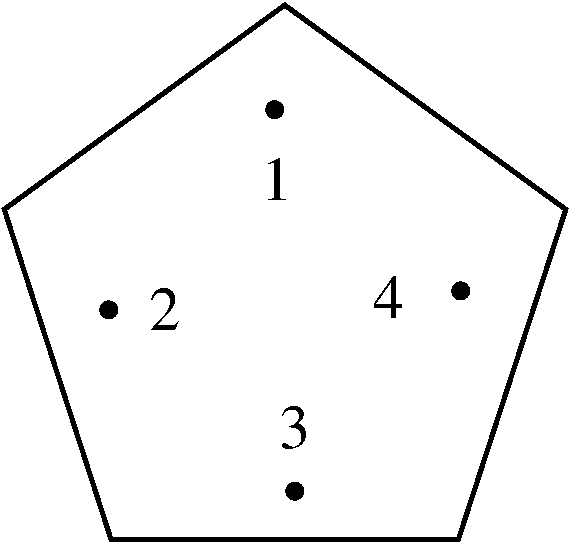
\includegraphics[width=4cm]{figures/pentagon_degree3.pdf}
    \hspace{1cm}
    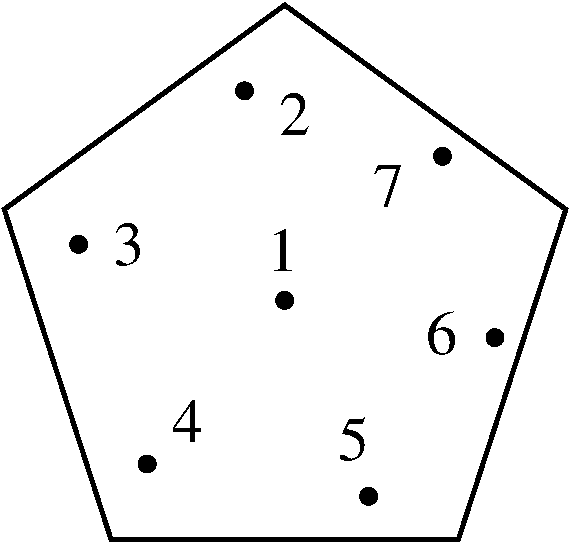
\includegraphics[width=4cm]{figures/pentagon_degree5.pdf}
    \caption{Locations of generalized, Gaussian, quadrature nodes for the $3^{\mathrm{rd}}$ (left) and $5^{\mathrm{th}}$ (right) degree integration methods presented in Table~\ref{tabQuadrature}.  Vertex 1 is located at the top of the pentagon, cf.\ Fig.~\ref{figRegPentagon}, while the coordinate origin is located at its centroid (node 1 in the right figure).}
    \label{figQuadrature}
\end{figure}

The Gaussian quadrature rules of Mousavi, Xiao \& Sukumar \cite{Mousavietal10} presented in Table~\ref{tabQuadrature} are compatible with the shape functions of Wachspress \cite{Wachspress75,Wachspress16} and Dasgupta \cite{Dasgupta03} presented in \S\ref{secShapeFns}.

\subsection{Gauss Integration of a Tetrahedron}

Integrating over the volume of a tetrahedron, when expressed in its natural co-ordinates $( \xi , \eta , \zeta )$, which span ranges of $0 \leq \xi \leq 1 - \eta - \zeta$, $0 \leq \eta \leq 1 - \zeta$ and $0 \leq \zeta \leq 1$, so that an integral of some function $f ( \xi , \eta , \zeta )$ becomes
\begin{multline}
     I = \int_0^1 \int_{\eta=0}^{1-\zeta} \int_{\xi = 0}^{1 - \eta - \zeta} 
     f ( \xi , \eta , \zeta ) \, \mathrm{d} \xi \, \mathrm{d} \eta \, 
     \mathrm{d} \zeta = \sum_{i=1}^n w_i f( \xi_i , \eta_i , \zeta_i ) + E \\
     \text{with} \quad 
     \int_0^1 \int_{\eta=0}^{1-\zeta} \int_{\xi = 0}^{1 - \eta - \zeta} 
     \mathrm{d} \xi \, \mathrm{d} \eta \, \mathrm{d} \zeta = \sum_{i=1}^n w_i = 
     \frac{1}{6}
\end{multline}
where co-ordinates $\xi_i$, $\eta_i$ and $\zeta_i$ place the $i^{\text{th}}$ node of integration inside a tetrahedron, and whose corresponding weight of integration is $w_i$, with there being $n$ pairs of nodes and weights.  The volume of this tetradedron is \textfrac{1}{6}.  Table~\ref{tabQuadraturetetra} provides a selection of quadrature rules for tetrahedra when expressed in their natural co-ordinate system.  This table can be found in some finite element textbooks.

\footnotesize
\begin{table}
    \hspace{-1.75cm}
    \begin{tabular}{|c|rrrr|}
        \hline
        node & \centering $\xi$ co-ordinate \phantom{12} & $\eta$ co-ordinate \phantom{12} & 
        $\zeta$ co-ordinate \phantom{12} & weight \phantom{12345} \\ \hline        
        & \multicolumn{4}{|c|}{Exact for Polynomials of Degree $1^{\phantom{|^|}}$} \\ 
        \hline
        1 & 0.250000000000000 & 0.250000000000000 & 0.250000000000000 & 
            0.166666666666667 \\ 
        \hline
        & \multicolumn{4}{|c|}{Exact for Polynomials of Degree $3^{\phantom{|^|}}$} \\ \hline
        1 & 0.250000000000000 & 0.250000000000000 & 0.250000000000000 & 
           -0.133333333333333 \\
        2 & 0.500000000000000 & 0.166666666666667 & 0.166666666666667 &  
            0.075000000000000 \\
        3 & 0.166666666666667 & 0.500000000000000 & 0.166666666666667 &  
            0.075000000000000 \\ 
        4 & 0.166666666666667 & 0.166666666666667 & 0.500000000000000 & 
            0.075000000000000 \\
        5 & 0.166666666666667 & 0.166666666666667 & 0.166666666666667 & 
            0.075000000000000 \\
        \hline
        & \multicolumn{4}{|c|}{Exact for Polynomials of Degree $5^{\phantom{|^|}}$} \\ \hline
        1 & 0.250000000000000 & 0.250000000000000 & 0.250000000000000 &    
            0.030283678097089 \\
        2 & 0.000000000000000 & 0.333333333333333 & 0.333333333333333 & 
            0.006026785714286 \\
        3 & 0.333333333333333 & 0.000000000000000 & 0.333333333333333 & 
            0.006026785714286 \\ 
        4 & 0.333333333333333 & 0.333333333333333 & 0.000000000000000 & 
            0.006026785714286 \\
        5 & 0.333333333333333 & 0.333333333333333 & 0.333333333333333 & 
            0.006026785714286 \\
        6 & 0.727272727272727 & 0.090909090909091 & 0.090909090909091 & 
            0.011645249086029 \\
        7 & 0.090909090909091 & 0.727272727272727 & 0.090909090909091 & 
            0.011645249086029 \\
        8 & 0.090909090909091 & 0.090909090909091 & 0.727272727272727 & 
            0.011645249086029 \\ 
        9 & 0.090909090909091 & 0.090909090909091 & 0.090909090909091 & 
            0.011645249086029 \\
        10 & 0.066550153573664 & 0.433449846426336 & 0.433449846426336 & 
             0.010949141561386 \\
        11 & 0.433449846426336 & 0.066550153573664 & 0.433449846426336 & 
             0.010949141561386 \\
        12 & 0.433449846426336 & 0.433449846426336 & 0.066550153573664 & 
             0.010949141561386 \\
        13 & 0.433449846426336 & 0.066550153573664 & 0.066550153573664 & 
             0.010949141561386 \\ 
        14 & 0.066550153573664 & 0.433449846426336 & 0.066550153573664 & 
             0.010949141561386 \\
        15 & 0.066550153573664 & 0.066550153573664 & 0.433449846426336 & 
             0.010949141561386 \\ 
        \hline
    \end{tabular}
    \caption{Symmetric weights and nodes for Gauss quadratures that integrate over a tetrahedron in its natural co-ordinate system $(\xi , \eta , \zeta)$, where $0 \leq \xi \leq 1 - \eta - \zeta$, $0 \leq \eta \leq 1 - \zeta$ and $0 \leq \zeta \leq 1$.  These weights sum to \textfrac{1}{6}, which is the volume of a tetrahedron measured in its natural co-ordinate system.}
    \label{tabQuadraturetetra}
\end{table}
\normalsize
